\chapter*{Ringraziamenti}
\addcontentsline{toc}{chapter}{Ringraziamenti}
\markboth{Ringraziamenti}
\emph{Siamo giunti alla conclusione di questo lavoro di tesi che chiude questo percorso di studi iniziato nel 2019 da un ragazzo che non sapeva nemmeno cosa fosse l’informatica, che, dopo il primo anno, dopo la pandemia, dopo aver avuto difficoltà a superare anche i primi esami, stava iniziando a pensare che forse non era la strada giusta per lui. Tuttavia, anche con l’aiuto di chi gli è stato vicino, oggi quel ragazzo si ritrova a festeggiare il raggiungimento di un traguardo che solo due anni fa sembrava irraggiungibile.

Il mio primo ringraziamento va a Dio; durante questo percorso di studi ho avuto modo di avvicinarmi alla fede e di conoscere il Signore personalmente. Questo mi ha portato, tra le tantissime cose positive, ad avere una spinta in più anche nell’ambito universitario; in Lui ho trovato la forza e il coraggio di andare avanti e di superare anche i momenti più difficili; ho sperimentato la Sua vicinanza e la Sua guida in ogni situazione e ho visto la Sua mano potente condurmi al meglio nel mio cammino. Nella Bibbia è scritto in Filippesi 4:6 “Non angustiatevi di nulla, ma in ogni cosa fate conoscere le vostre richieste a Dio in preghiere e suppliche, accompagnate da ringraziamenti”; durante questo percorso ho pregato tanto Dio ed Egli mi ha risposto e, in virtù di questo, non voglio dimenticare anche la seconda parte del versetto appena citato, ringraziandoLo, appunto, per ogni cosa che Egli ha fatto per me.

Voglio ringraziare anche il Prof. Ursino; sin dal primo giorno di lezione mi ha fatto appassionare tanto all’Ingegneria del Software; nonostante le difficoltà a superare l’esame, ha saputo affrontare la situazione particolare che si era creata e, venendomi incontro, mi ha aiutato nella consegna del progetto finale, nonché il mio primo software sviluppato. Nel corso del lavoro di tesi, poi, è stato sin da subito molto disponibile e gentile nei miei confronti, nonostante mi trovassi in una situazione nuova e non sapevo bene come muovermi; è stato sempre puntuale sia nelle risposte alle mie domande sia nelle correzioni, rendendo questa esperienza piacevole, leggera, senza affanni e preoccupazioni, ma allo stesso tempo molto professionale. Ho apprezzato molto il suo modo di rapportarsi con me; solo il fatto di essere addirittura chiamato per nome (e che bel nome!) mi ha fatto sentire molto coinvolto e vicino; quando mi parlava, sembrava quasi si rivolgesse non a uno studente, ma ad un figlio e questa è una cosa che ho apprezzato tanto.

Voglio ringraziare i miei genitori, mamma e papà, che mi hanno sempre sostenuto, incoraggiato, mi sono sempre stati vicini e sono stati pronti tanto a festeggiare per gli esami superati, quanto a tirarmi su nei momenti di difficoltà. Non mi hanno fatto mai mancare niente, sia dal punto di vista materiale che, soprattutto, morale, concedendomi di vivere un’esperienza fantastica sotto ogni punto di vista. Vivere lontano dalla propria famiglia non è semplice, sia per noi figli, ma anche per i genitori, e questo l'ho capito nel corso di questi anni. Nonostante la lontanaza, però, mamma e papà hanno sempre avuto a cuore di sentirmi, giorno dopo giorno, attraverso le videochiamate quotidiane e, quando c'è stata l'opportunità, anche venendomi a trovare, addirittura a sorpresa una volta, qui ad Ancona. Quando si va a vivere da soli, si capiscono tante cose e si inizia a dare valore a molti aspetti su cui prima non ci si soffermava abbastanza; è stato proprio questo quello che è successo: ho iniziato a dare valore ai momenti trascorsi in famiglia, che prima erano scontati, ma ora sono diventati molto meno frequenti; ho apprezzato ancora di più i sacrifici fatti da mamma e papà nel portare avanti una famiglia, sotto ogni punto di vista; in questa mia esperienza da fuori sede ho imparato talmente tanto ad empatizzare con i sacrifici fatti dai miei genitori che ho iniziato ad utilizzare frasi del tipo: "Ho appena pulito e già è sporco!" oppure "La luce accesa consuma corrente!". Posso dire che ho iniziato a dare tanto valore a cose che prima, probabilmente, davo per scontate, ma che, in realtà, non lo erano per niente. Ed è per questo che ci tengo ancora a ringraziare mamma e papà per tutto quello che hanno fatto per me, non soltanto in questi anni, ma in tutta la mia vita.

Voglio ringraziare i miei fratelli Michele e Marco; ognuno dei due, in una maniera diversa, visti gli anni di differenza, mi ha aiutato in questi anni. Con Michele ho avuto il piacere di vivere nella stessa casa per tre anni; trascorrere le giornate lontano dal proprio paese e dai propri genitori non è semplice, ma la presenza costante di un fratello, così come l’ho avuta io, ha reso tutto molto più leggero e semplice, come se, alla fine, casa nostra non l’avessimo mai lasciata. Marco è il fratellino piccolo a cui vorresti insegnare tutto quello che impari, sperando di trasmettergli gli stessi interessi; per ora non ci sono riuscito: infatti ha sempre storto il naso quando volevo fargli testare i programmi che sviluppavo; però vedere la sua spensieratezza, quella di un bambino, vedere anche la sua gioia, sincera, quando tornavo a trovarlo o quando lui veniva a visitarmi qui ad Ancona, ma anche il suo dispiacere quando ripartivo, mi ha aiutato veramente tanto.

Voglio ringraziare tutto il resto della mia famiglia, i miei nonni Mimì, Rita, Michele e Maria, i miei zii Matteo, Lucia, Patrizia, Lucia, Vincenzo, le mie cugine Valentina, Rita, Ciretta; tutti, in un modo diverso, sono stati importanti in questo percorso.

Voglio ringraziare Maria Chiara, una delle persone per me più importanti e che più ha avuto un'impronta in questi anni, dimostratomi, in tante occasioni, la sua vicinanza e il suo affetto. Voglio ringraziare Miriana, un’altra presenza costante in questo mio percorso, che mai ha fatto mancare in me il suo sostegno in ogni circostanza, sempre pronta in qualsiasi momento ad essere presente. Voglio ringraziare Andrea, il fratello maggiore che non ho mai avuto, un esempio per me, una persona che mi ha dato tanto, forse anche più di quello che crede. Voglio ringraziare Angela, colei che, dopo averla conosciuta nel mio paese d’origine quando ero bambino, ho rincontrato dopo più di dieci anni qui ad Ancona e che, da quel momento in poi, ha sempre ricoperto un ruolo molto importante.

Voglio ringraziare Giuseppe, la prima persona che mi ha rivolto la parola all’università, il mio collega nello sviluppo di GreenMarket, ma, soprattutto, un amico con cui ho condiviso quotidianamente tutto il mio percorso universitario. Voglio ringraziare Emanuele, la prima macchina da guerra, dal punto di vista della programmazione, conosciuta; ricordo con piacere CovidForecast, progetto di Programmazione ad Oggetti, ed è vedendolo lavorare in quel contesto che ho iniziato ad apprezzare lo sviluppo di programmi, la creazione di interfacce grafiche la programmazione in generale. Voglio ringraziare Paolo, un altro programmatore fuori dal comune che, a vederlo lavorare su FlatMate, ho avuto solo da prendere esempio. Voglio ringraziare Emilio, con cui non ho mai lavorato insieme, ma ho avuto modo di vedere quanto fosse in gamba e professionale sotto ogni punto di vista. A prescindere, però, dalle competenze, loro sono stati gli amici con cui ho condiviso ogni momento nell’ambito universitario, sin dalle prime esercitazioni di Algebra Lineare e Geometria del lontano settembre 2019 e li ringrazio per essere sempre stati presenti in ogni contesto.

Voglio ringraziare Giovanni, il mio amico, ormai fratello, con cui ci conosciamo da 21 anni. Abbiamo condiviso insieme gli anni dall’asilo fino alle scuole superiori; poi, purtroppo, le strade si sono separate; nonostante i 300km di distanza, però, siamo sempre stati vicini, anche durante il percorso universitario e, ogni volta che ci rincontravamo, era come se non ci fossimo mai lasciati.

Voglio ringraziare tutto il mio gruppo di amici del mio paese di origine; anche se siamo andati a finire in zone diverse dell’Italia, siamo sempre rimasti in contatto; inoltre, non dimentico i caffè presi e le chiacchierate fatte quando ci rincontravamo, momenti preziosi che ho sempre apprezzato tanto.

Voglio ringraziare il gruppo giovani della chiesa di San Nicandro Garganico; ognuno in una maniera diversa, sono stati, a partire dal 2021, anno in cui mi sono legato maggiormente a loro, una presenza importantissima; sapere che in ogni occasione avrei trovato il loro appoggio e il loro sostegno mi ha dato una grande mano, e per questo voglio ringraziarli.

E per ultimo, non posso dimenticare di ringraziare l’Impresa Edile La Porta Tommaso che, nelle figure di mio padre e di mio nonno, mi ha dato anche l’opportunità, come si vede nelle Figure \ref{io}, \ref{nonnomimi}, \ref{marco}, \ref{michele} e \ref{michele2}, di sporcarmi le mani durante la fase di specifica dei requisiti; ciò mi ha aiutato nella realizzazione del software, in quanto mi ha fatto comprendere ancora meglio i processi aziendali :D.

Concludo con un grazie complessivo a chiunque abbia avuto un ruolo in questo mio percorso. Grazie a tutti voi. 

\begin{figure}[ht!]
	\centering
	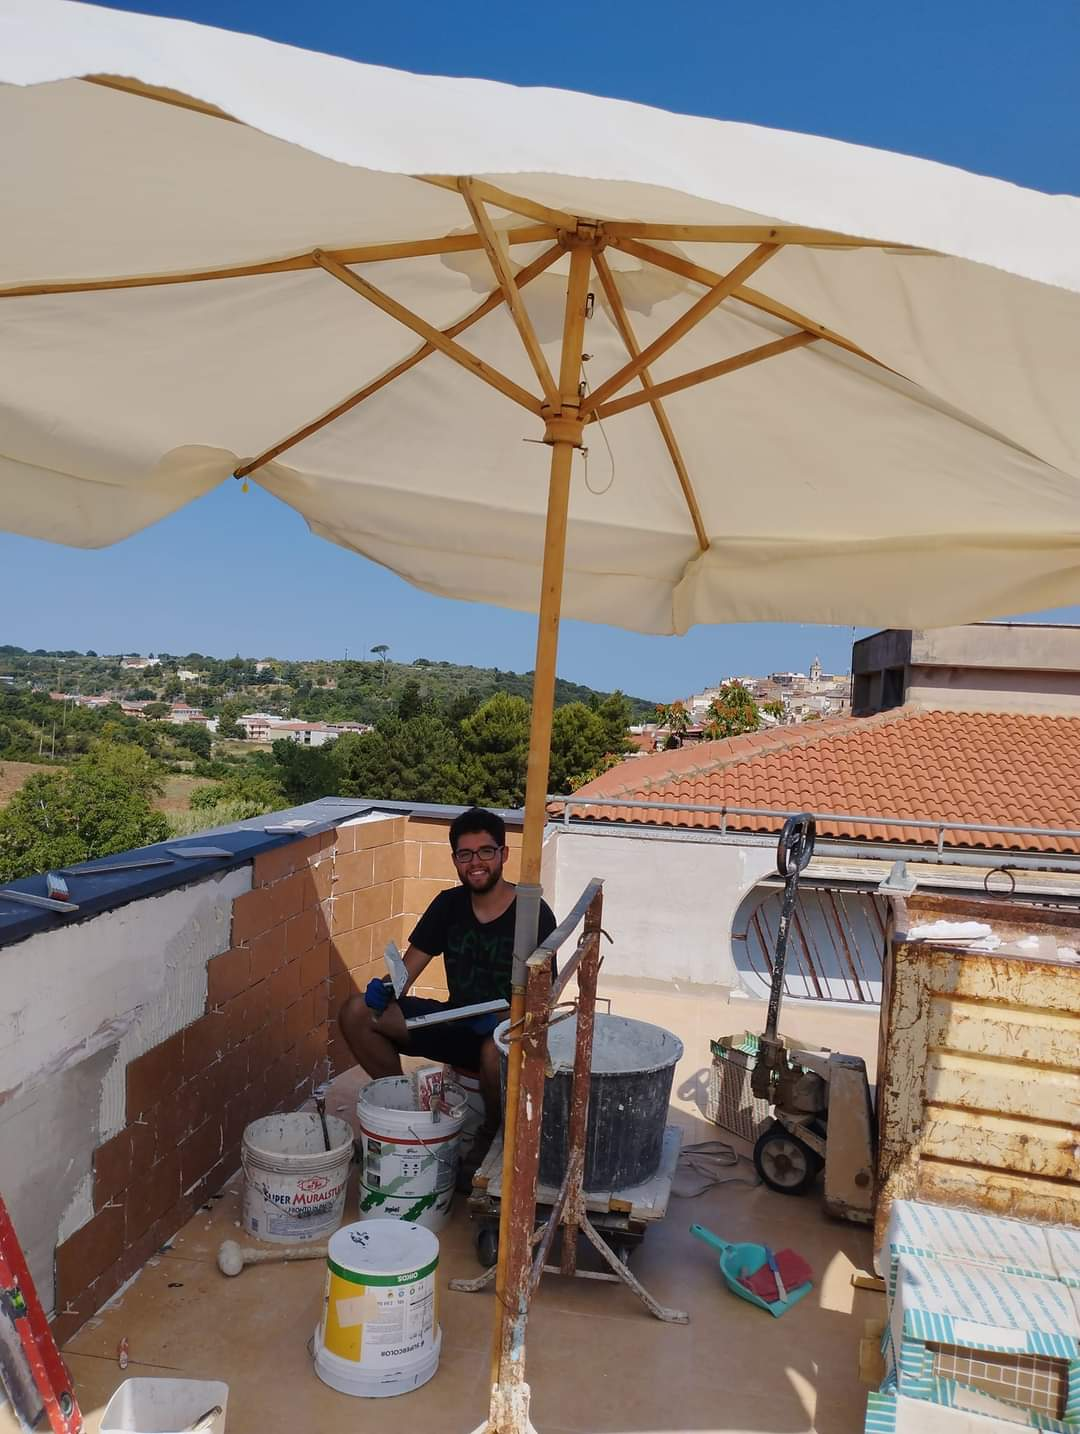
\includegraphics [width=0.75\columnwidth, angle=0]{acknowledgements/images/fotomia.jpg} % height
	\caption{Foto in cantiere da solo}
	\label{io}
\end{figure}

\begin{figure}[ht!]
	\centering
	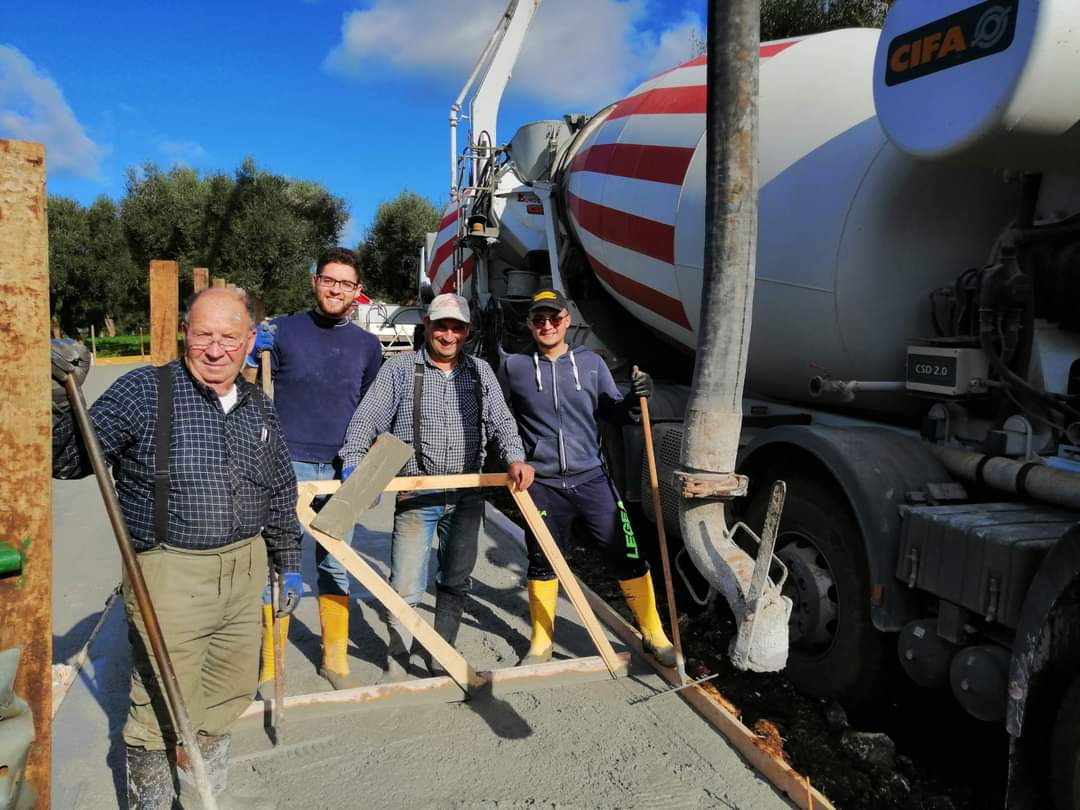
\includegraphics [width=0.85\columnwidth, angle=0]{acknowledgements/images/fotoconnonnomimi.jpg} % height
	\caption{Foto in cantiere con nonno Mimì, papà e mio fratello Michele}
	\label{nonnomimi}
\end{figure}

\begin{figure}[ht!]
	\centering
	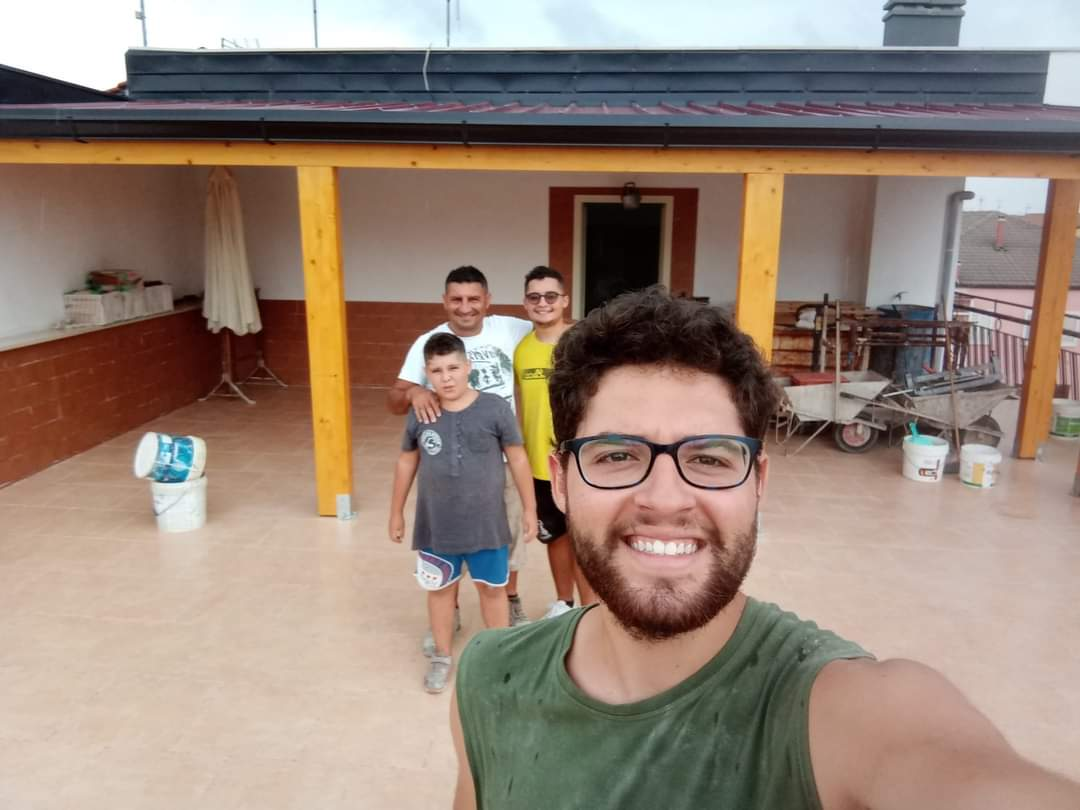
\includegraphics [width=0.85\columnwidth, angle=0]{acknowledgements/images/fotoconmarco.jpg} % height
	\caption{Foto in cantiere con papà e i miei due fratelli Michele e Marco}
	\label{marco}
\end{figure}

\begin{figure}[ht!]
	\centering
	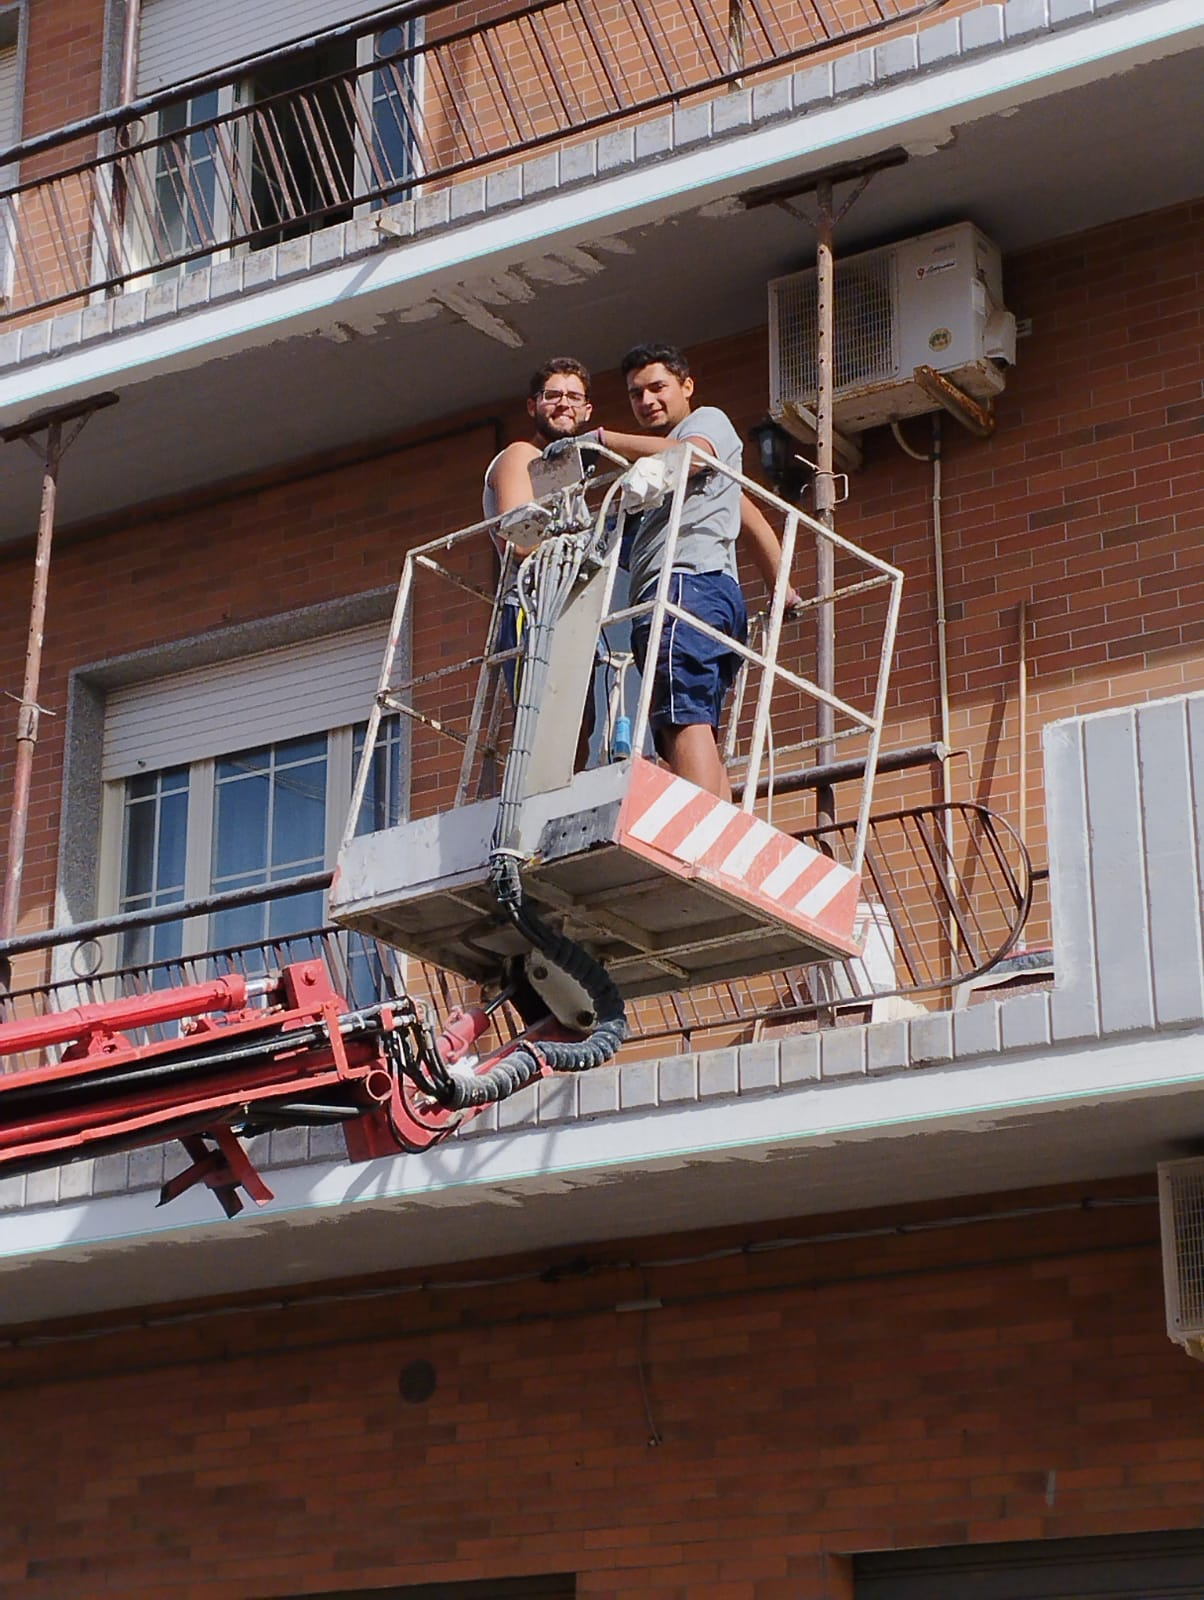
\includegraphics [width=0.75\columnwidth, angle=0]{acknowledgements/images/foto_com_michele.jpeg} % height
	\caption{Foto sul cestello con mio fratello Michele}
	\label{michele}
\end{figure}

\begin{figure}[ht!]
	\centering
	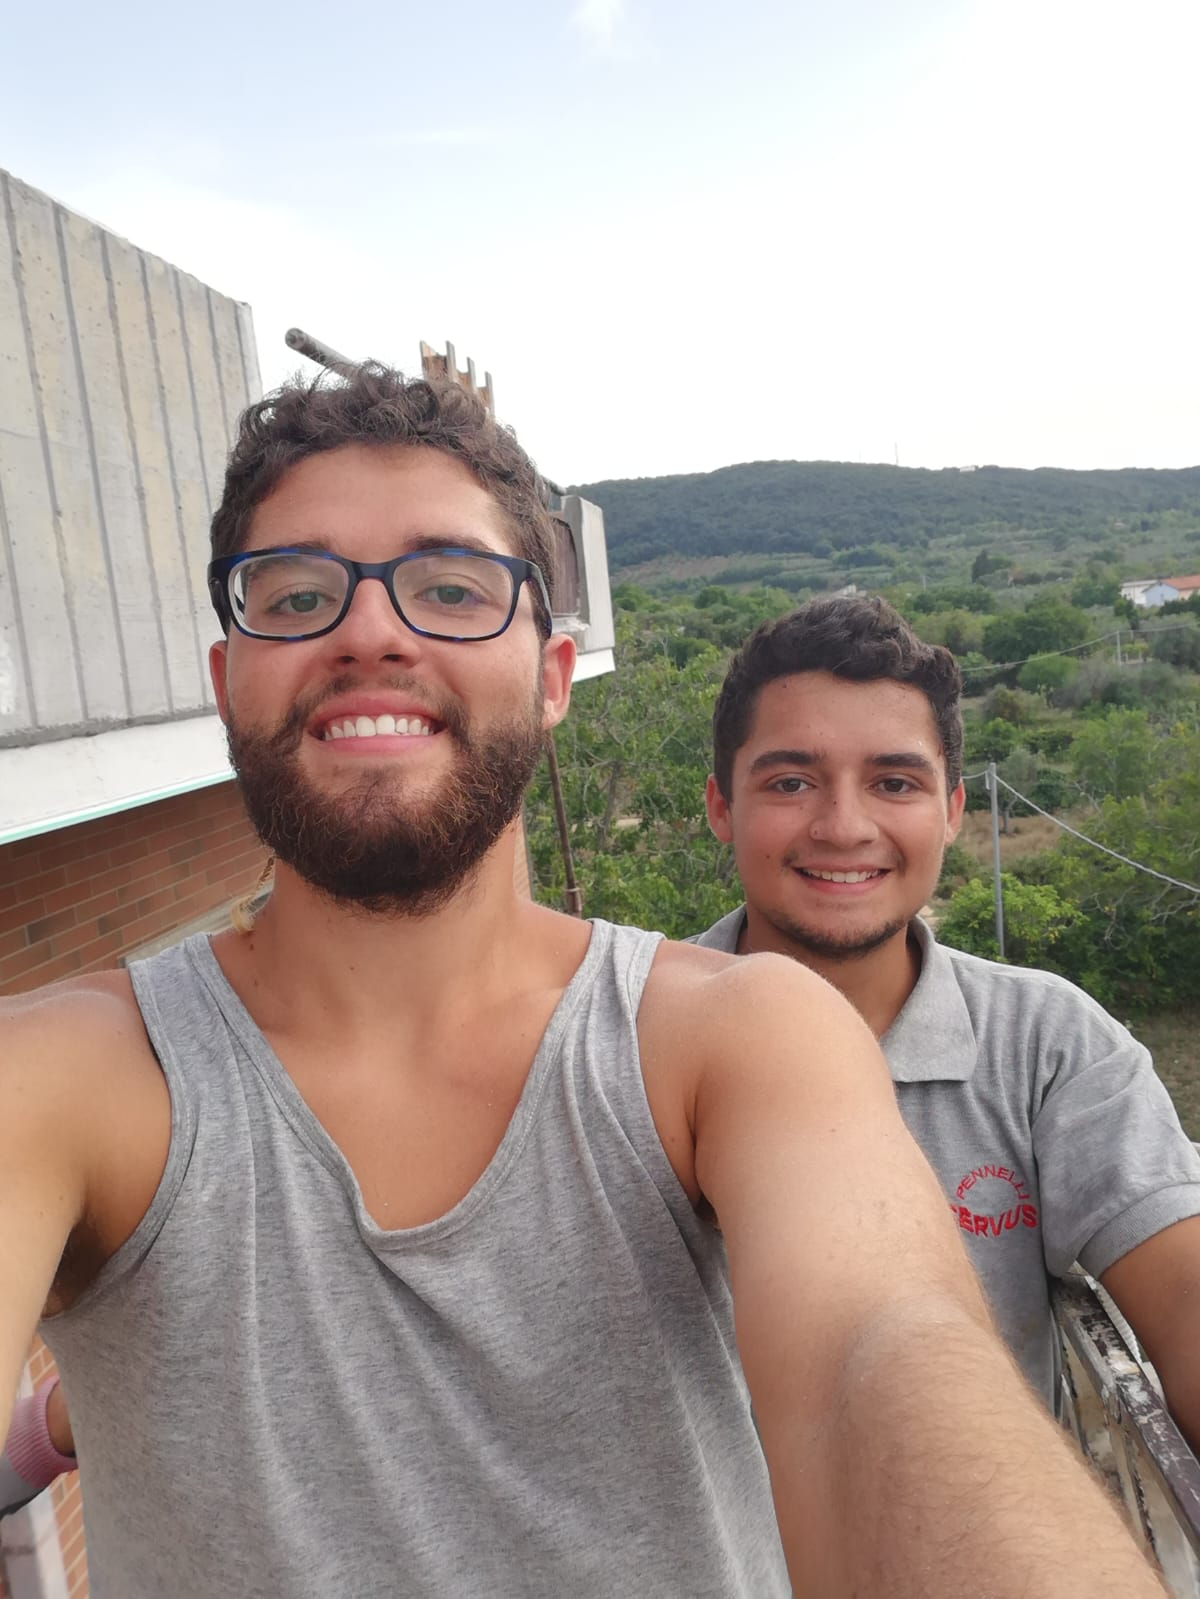
\includegraphics [width=0.75\columnwidth, angle=0]{acknowledgements/images/foto_sul_cestello.jpeg} % height
	\caption{Foto in cantiere con mio fratello Michele}
	\label{michele2}
\end{figure}

}